
% 两列环境示例
\section{多列布局}
\begin{frame}
\frametitle{两列环境示例}
\begin{columns}
\column[t]{0.5\textwidth}
在这个示例中,我们将展示如何使用两列环境来并排显示内容。这种方法在需要对比不同信息或并排显示文本和图像时非常有用。

例如,我们可以在这边列出一些优点:
\begin{itemize}
  \item 节省空间
  \item 便于对比
  \item 增强可读性
\end{itemize}

\column[t]{0.5\textwidth}
同时在另一边列出一些缺点:
\begin{itemize}
  \item 可能显得拥挤
  \item 需要仔细平衡内容
  \item 在小屏幕上可能显示不佳
\end{itemize}

也可以放置图像或者公式等内容。
\end{columns}
\end{frame}

% 包含图片、表格和tikz绘图的多列示例
\begin{frame}
\frametitle{多列环境:图片、表格和TikZ绘图示例}
\begin{columns}[T]
\column{0.33\textwidth}
\centering
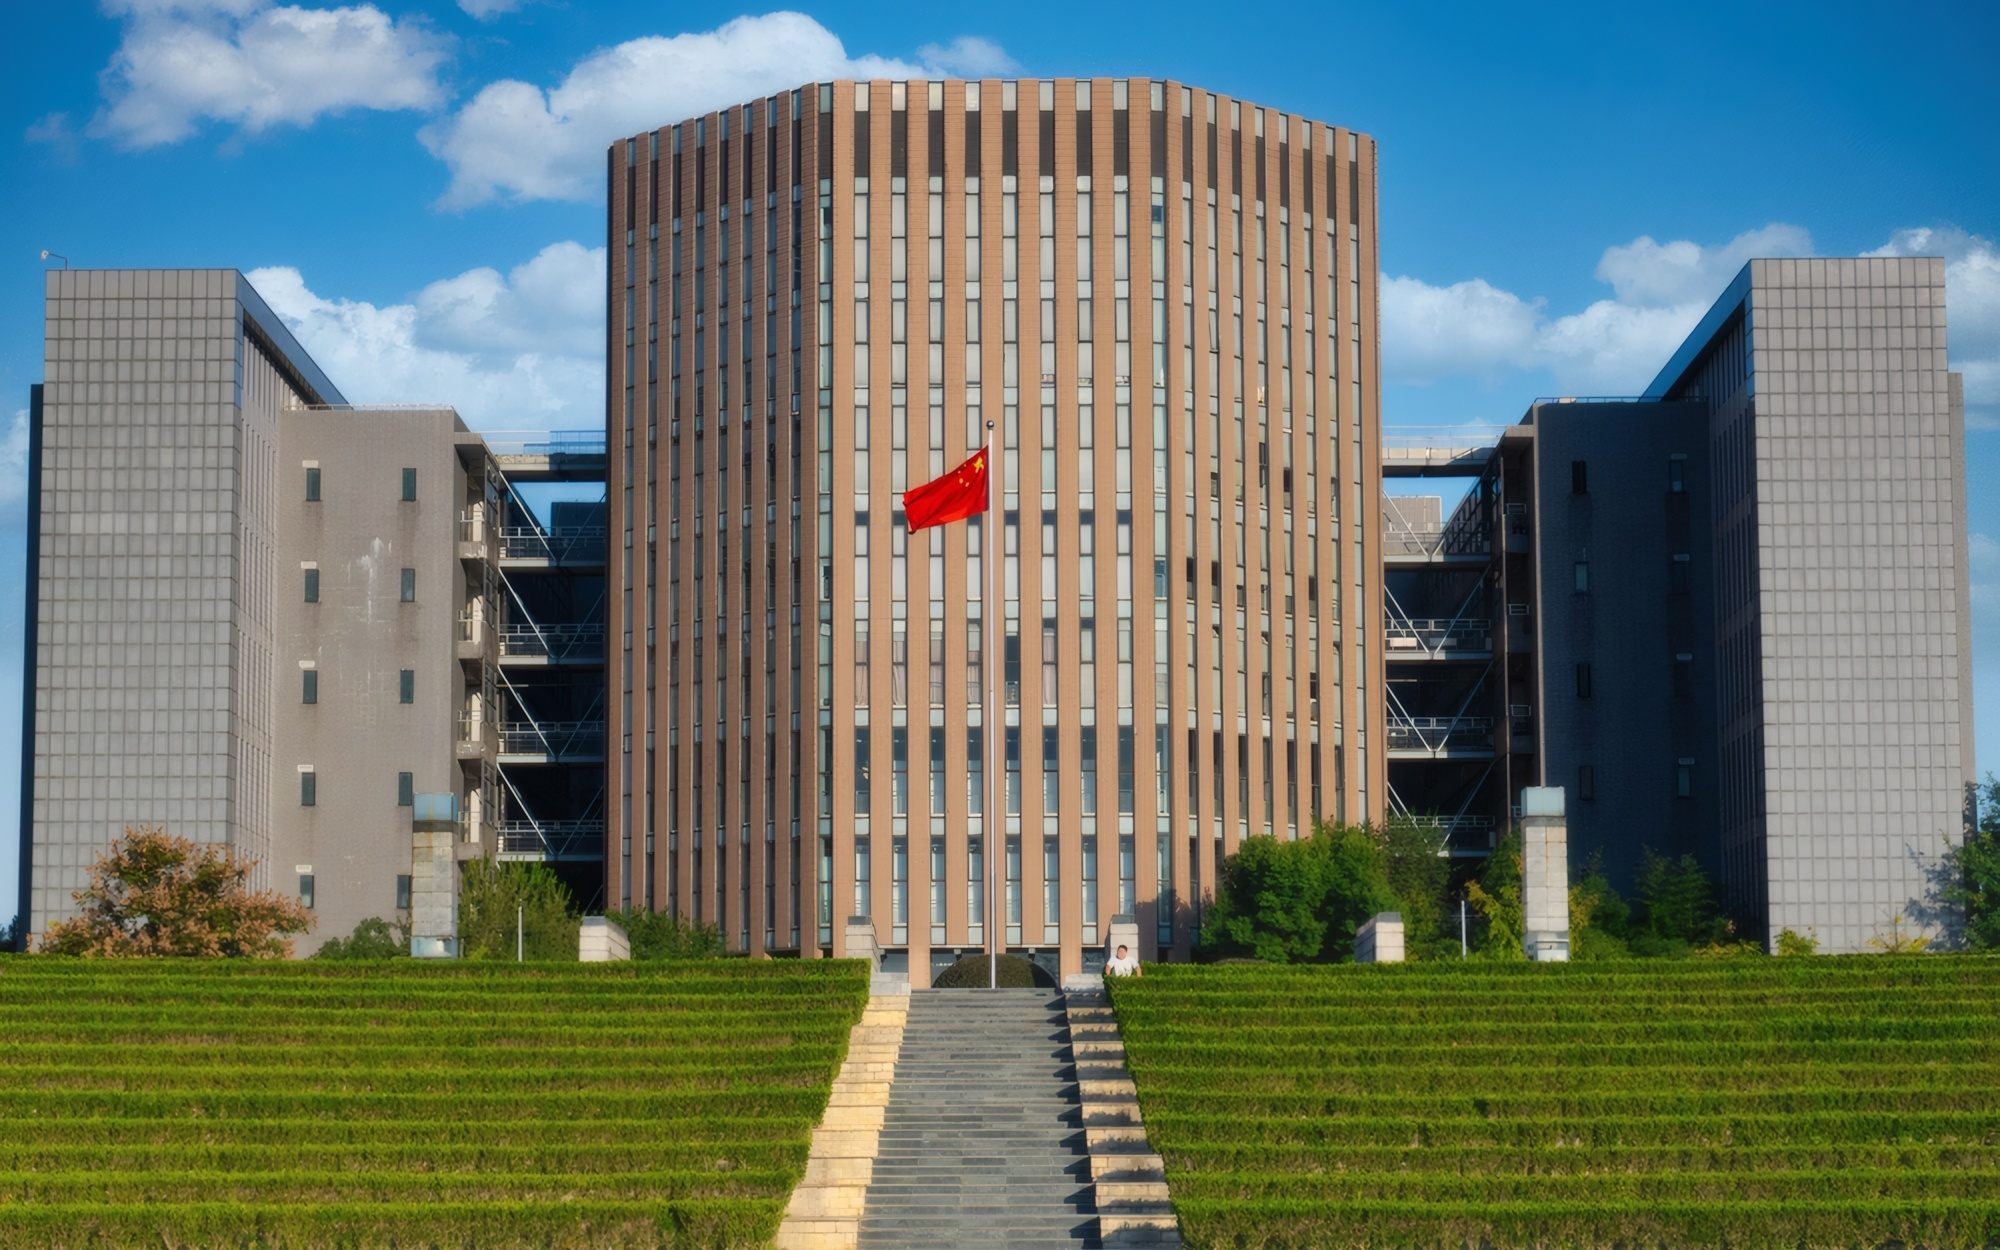
\includegraphics[width=0.7\linewidth]{src/example_ahu.jpg}

\vspace{1em}

\parbox[t]{\linewidth}{
\raggedright
示例图片说明文字\\
这是对图片内容的简要描述
}

\column{0.33\textwidth}
\centering
\begin{tabular}{|c|c|}
\hline
A & B \\
\hline
1 & 2 \\
3 & 4 \\
\hline
\end{tabular}

\vspace{1em}

\parbox[t]{\linewidth}{
\raggedright
示例表格说明文字\\
这是对表格内容的简要描述
}

\column{0.33\textwidth}
\centering
\begin{tikzpicture}
\draw[thick] (0,0) rectangle (1.5,1);
\draw (0.75,0.5) node {示例};
\end{tikzpicture}

\vspace{1em}

\parbox[t]{\linewidth}{
\raggedright
TikZ绘图说明文字\\
这是对绘图内容的简要描述
}
\end{columns}
\end{frame}